\documentclass{aa}
\usepackage[varg]{txfonts}
\usepackage{graphicx}       % Include figure files
\usepackage{amsfonts,amsmath}
\usepackage{natbib}
%%%%%%%%%%%%%%%%%%%%%%%%%%%%%%%%%%%%%%%%%%%%%%
% Sarp's commands
\newcommand{\be}{\begin{equation}}
\newcommand{\ee}{\end{equation}}
\newcommand{\f}{\frac}
\newcommand{\nn}{\nonumber}
%%%%%%%%%%%%%%%%%%%%%%%%%%%%%%%%%%%%%%%%%%%%%%
%%%%%%%%%%%%%%%
%%%%%%%%
%%%
%
\begin{document}
\title{
%Forecasting Gamma-Ray Bursts with Gravitational-wave Detectors
Electromagnetic follow-ups in the era of forecasting gamma-ray bursts
%\thanks{Grant1}\fnmsep
%\thanks{Grant2}\\
}
\subtitle{Subtitle here if needed}
\author{Sarp Akcay\inst{1}\inst{2}
\and Antonio Martin-Carrillo\inst{3}
\and Morgan Fraser\inst{3}}
%\thanks{\emph{Present address:}
%Department of Computer Science, Purdue University,
%West Lafayette, IN 47907, USA}

\institute{Theoretisch-Physikalisches Institut, Friedrich-Schiller-Universit{\"a}t Jena, 07743, Jena, Germany
\and School of Mathematics \& Statistics, University College Dublin, Belfield, Dublin 4, Ireland
\and School of Physics, University College Dublin, Belfield, Dublin 4, Ireland} % Space Science Group,
% \date{Received 2 November 2018 / Accepted 7 January 2018}
\abstract{
The detection of gravitational waves from the binary neutron star inspiral-merger event GW170817 and the subsequent
extended electromagnetic follow-up observations of the resulting kilonova
gave us a small taste of multi-messenger astronomy across the spectra of \emph{two} fundamentally
different kinds of radiation.
The opportunities to conduct such multi-disciplinary study will increase by two orders of magnitude
in the 2030s with Einstein Telescope, LIGO's European successor.
Due to its extreme sensitivity in the $1-10\,$Hz regime, the Einstein Telescope's C configuration (ET-C) will be capable of detecting inspiralling binary neutron star systems out to luminosity distances of 1 Gpc.
For inspirals within half of this distance
ET-C will accumulate signal-to-noise ratios of $\gtrsim 15$ %and localize the source to $\lesssim \mathcal{O}(10)\,\text{deg}^2$ 
with more than an hour left to merger. 
However, the localization of ET alone is rather poor: within $z=0.1$ we expect to have $\sim 5 $ BNSs to be localized to $\Delta\Omega\lesssim 10\,$deg$^2$.
On the other hand, a second less sensitive gravitational-wave detector (such as future KAGRA)
%GW detector with just ten times KAGRA sensitivity at 5\,Hz 
would increase the number of well-localized sources to $\mathcal{O}(100)$.
Thus it is imperative to have at least one companion detector to ET with significantly improved seismic isolation in the 2030s.
Having numerous GW sources localized to $\sim10\,$deg$^2$ opens the possibility of doing detailed follow-up observations of
the resulting kilonovae with ATHENA, LSST, BlackGEM ...
Here we explore this intriguing possibility...
Thus, this letter is an appeal/plea(?) to the astronomy community to have in place ...

%We explore the  possibility of employing future ground-based gravitational-wave interferometers to detect the inspiral of binary neutron stars sufficiently
%early to alert electromagnetic observatories so that a gamma-ray burst (GRB) can be observed in its entirety from its very beginning.
%We quantify the ability to predict a GRB by computing the time a binary neutron star (BNS) system takes to inspiral from its moment of detection to its final merger. We define the moment of detection to be the instant at which the inteferometer network accumulates a signal-to-noise ratio of 15. %for the BNS inspiral.
%For our computations, %of advance warning times, 
%we specifically consider BNS systems at luminosity distances of (i) $D\le200\,$Mpc in the three-interferometer Advanced-LIGO-Virgo network of 2020, and (ii) $D \le 1000\,$Mpc in the Einstein Telescope's B and C configurations. 
%In the case of Advanced LIGO-Virgo we find that we may at best get a few minutes of warning time, thus we expect no forecast of GRBs in the 2020s. 
%On the other hand, Einstein Telescope will provide us with advance warning times of more than five hours for $D \le 100\,$Mpc.
%Taking one hour as a benchmark advance warning time, we obtain a corresponding horizon
%distance of roughly 600 Mpc for the Einstein Telescope C configuration.
%Using current BNS merger event rates within this volume, we show that Einstein C will forecast $\gtrsim \mathcal{O}(10^2)$ GRBs in the 2030s. %with Einstein C. %with the C configuration of Einstein Telescope.
%We reapply our warning-time computation to binary black hole - neutron star inspirals and find that we expect 1 to 3 tidal disruption events to be forecast by the same detector.
}
\keywords{gravitational waves --gamma-ray bursts -- kilonovae}
\maketitle

\section{Introduction}

Gravitational waves offer a unique insight into some of the most extreme physical processes in the Universe - including the merger of black holes (BH) and neutron stars (NS), and the first seconds of core-collapse supernovae explosions. 

With the first direct detection of gravitational waves (GWs) in 2015 by the Advanced Laser Interferometer Gravitational-Wave
Observatory (Advanced LIGO; \citealp{FirstGW}), gravitational wave astronomy moved from prospect to reality. The first GW source observed by Advanced LIGO, GW150914, matched the signal predicted for the merger of two black holes with masses 36 and 29 M$_{\odot}$. Along with being the first direct detection of GWs, GW150914 was also the first detection of such heavy black holes, which had significantly larger masses compared to those measured for Galactic high mass x-ray binaries. Such massive black holes provide an interesting constraint on stellar evolutionary channels at low metallicity \citep[e.g.][]{FirstGW_astro, Belc16}. While no electromagnetic counterpart is generally expected to accompany the merger of two black holes, an intensive multi-wavelength search of the probable location of GW150914 was carried out \citep{FirstGW_EM}. Despite yielding a null result, this effort served as a rehearsal in preparation for searches for counterparts to GW sources that {\it are} expected to be accompanied by an electromagnetic (EM) source.

Only two years after the first detection of merging black holes by Advanced LIGO, both Advanced LIGO and the Virgo gravitational wave observatories detected GW170817, with waveform consistent with the merger of two neutron stars \citep{GW170817}. A spatially and temporally coincident short Gamma Ray Burst (GRB) was also seen by the {\it Fermi} and {\it INTEGRAL} satellites \citep{GW170817_GRB}. This discovery sparked a global effort to find the counterpart of GW170817 at optical wavelengths, which resulted in the identification of AT2017gfo less that 11 hours later \citep{GW170817_EM}. AT2017gfo faded exceptionally rapidly, and displayed cool temperatures and lines from unusual r-process elements at exceptionally high velocities \citep{Smar17,Arca17,Pian17,Coul17,Kilp17}. These characteristics marked AT2017gfo as a kilonova; a transient powered by the radioactive decay of short-lived nuclides formed in the merger of two neutron stars.

{\bf MF: Something about astrophysical significance of GW detections here. Cosmology. Localising KNe means we can study emission as a function of viewing angle - need large samples for this. Measurement of KN rate - need to get z?}

The identification of AT2017gfo as the counterpart to GW170817 was realised by the 
ability of Advanced LIGO-Virgo to localise the GW signal to $\sim$30 deg$^2$.
%small region on the sky ($\sim$30 deg$^2$) within which the GW was localised. 
In addition, at only 40 Mpc, GW170817 was exceptionally close. This enabled the EM counterpart to be identified through targeted observations of galaxies which were at this distance within the GW localisation region \citep{Coul17}. Unfortunately such a strategy is only feasible for the nearest GW sources, and rapidly becomes unfeasible beyond $\sim100-200$ Mpc, both as the number of galaxies within the search volume increases, and as the fraction of galaxies with reliable redshifts decreases. 
This embarrassment of riches becomes a serious obstacle for identifying EM counterparts to GW transients in the 2030s with Einstein Telescope becoming operational \citep{ET_doc}.

Einstein Telescope will be sensitive enough to ``pick up'' GW sources at a few Hz thanks to
its cryogenic design and underground housing which will shield it from low-frequency contaminants such as seismic and gravity-gradient noises. Moreover, ET will consist of three
 V-shaped interferometers which eliminate blind spots and further allow it to construct a null
 stream \citep{Sathyaprakash:2012jk} which can be used to veto spurious events \citep{Wen:2005ui}. 
 Additionally, ET will be a xylophone ({\bf cite?}), i.e., a multi-band detector capable of delivering high sensitivities both at low frequencies ($\sim 5\,$Hz) and high frequencies ($\sim 100\,$Hz). 
 %as we show in .
 Here, we focus on the C configuration (ET-C) which offers the highest low-frequency sensitivity as shown in Fig.~\ref{fig:ETB2030}.
 ET-C will detect $\gtrsim\mathcal{O}(10^3)$ BNS inspirals per year out to 1000Mpc with SNRs $\gtrsim 30 $ \citep{Akcay18}. A subset of these sources will be close enough that they will be detected a few hours
before their respective mergers \citep{Akcay18}, hence opening up the possibility of alerting EM
observatories to conduct follow-up observations \emph{before, during} and after the prompt gamma-ray bursts. Additionally, ET-C will forecast a few yearly potential tidal disruption events in which
a neutron star gets tidally torn by a $\sim 5 M_\odot$, high-spin black hole companion.
%{\bf Morgan:} should we add more details here such as specific numbers for events/year? I was
%leaving these for Sec. 2

%{\bf Something on future GW observatories - introduce Einstein Telescope etc. How many events do we expect to see per year? What at the timescales for these coming online}

To fully exploit the prospect of multi-messenger astronomy, a number of wide-field survey telescopes are either operational, in commissioning, or under construction. Foremost among these is the Large Synoptic Survey Telescope \citep[LSST;][]{LSSTbook}, which has an 8.4~m primary mirror, and will image 3.5 deg$^2$ in a single pointing. Construction of LSST is well underway, and the telescope is expected to begin full survey operations at the start of 2023. Apart from LSST, the majority of current and next-generation survey telescopes have a relatively small mirror, but a large camera, and are designed to observe $\sim10 - 50$ sq degrees in a single pointing to a limiting magnitude of $\sim20-22$. ZTF \citep{ZTF}, GOTO \citep{GOTO} and ATLAS \citep{ATLAS} are all currently operational at present, while BlackGEM is currently under construction \citep{BlackGEM}.

{\bf Discuss search strategies discussed in literature - e.g. weighting by galaxy mass etc. Bottleneck is spectroscopic classification.}

%{\bf Intro to rest of paper. Our novel contribution is that we get an early warning for GWs. Can then use this to get templates immediately prior to the GW detection. Outline rest of section.}

Our aim here is to demonstrate exciting EM follow-up studies that can be done by taking advantage of the early GW warning capability of ET. More specifically we
consider binary neutron star inspirals
out to luminosity distances of $\sim 600\,$Mpc, 
the expected range of LSST. Within this range,
ET-C will be able to detect the inspiral GWs
a few hours before a given merger thus provide
a window of opportunity for mobilizing the EM
observatories in time to witness the birth of 
the associated kilonova. However, in order to
fully benefit from ET's early warnings, several
issues must be addressed: (i) ET's poor localisation by itself, (ii) large number of 
supernovae creating a confusion background, 
(iii) the slow response time of certain EM 
observatories essential to follow-up such as ATHENA, BLACKGEM {\bf Antonio, Morgan, is this right?}
Here, we consider each of these setbacks and
suggest solutions which require support from the global astronomy community.

This letter is organized as follows: Sec.~\ref{sect:et} provides more details on ET,
Sec.~\ref{sect:EM} investigates the implications
of optical follow-up. Sec.~4 ...
We use $f$ to denote the quadrupole GW frequency
in the detector frame. $c$ is the speed of light and $G$ is Newton's constant.
\section{Einstein Telescope}
\label{sect:et}
Consider a BNS system with component masses
$m_1, m_2$. For GW frequencies of interest to us here ($f \lesssim 10\,$Hz), the binary is undergoing an adiabatic inspiral dominated by
the emission of leading-order (quadrupole)
gravitational radiation. By balancing the
power emission in GWs to the rate of change of binding energy, we obtain the frequency evolution of the GW frequency
%
\be
\dot{f} = \f{96}{5}\pi^{8/3} \f{(G M_c)}{c^5}^{5/3}\, f^{11/3}, \label{eq:fdot}
\ee
where $M_c  = {(m_1 m_2)^{3/5}}{(m_1+m_2)^{-1/5}} $ is the chirp mass.
After fixing an integration, Eq.~\ref{eq:fdot}
can be integrated to yield the time left to merger at a given frequency, usually called the inspiral time
%
\begin{align}
\tau_\text{insp}(f) &= \f{5}{256\pi}\f{c^5}{(\pi G M_c)^{5/3}} \,f^{-8/3}\nn\\
&=16.72\,\text{minutes} \, \left(\f{1.219 M_\odot}{M_c}\right)^{5/3}\,\left(\f{10\,\text{Hz}}{f}\right)^{8/3}
\label{eq:tau_insp}\, ,
\end{align}
%



\begin{table}[h]
 \caption{Horizon distances of ET-B and ET-C assuming $T_\text{AW} =1\,$hour. $R(D_H)$ is the BNS merger rate within a volume of $D_H^3$
obtained by rescaling the rate inferred from Advanced LIGO's O1, O2 observing periods cite{GW170817}. $\bar\rho_F(D_H)$ is the total SNR accumulated due to a BNS inspiralling at $D_H$ [see Eq.~()].}
\label{table:horizon}
\centering
\begin{tabular}{l|ccc}
\hline
 & ET-B & & ET-C\\
\hline
  $D_H $& 87\,Mpc& &{613\,Mpc}\\
  $R(D_H) $& $1^{+2}_{-1}\,\text{yr}^{-1}$&\hspace{5mm} &{$355^{+730}_{-280}\,\text{yr}^{-1}$}\\
  $\bar\rho_F(D_H)$ & 420 &&{58}\\
\hline
\end{tabular}
\end{table}

\begin{table*}[h]
\caption{Forecasting capabilities of Einstein Telescope summarized. 
ET-B and ET-C refer to the different configurations shown in Fig.~. For the advance warning times, we only present the result of the more accurate 3.5PN computation. $\bar{f}_\text{ET}$ is the threshold frequency at which
ET-B/C accumulate SNR of 15 which we take to be our detection criterion. Note that both $T_\text{AW}$ and $\bar\rho_F$ are larger for ET-C
due to its improved sensitivity in the $1\,\text{Hz}\lesssim f\lesssim 30\,$Hz regime compared to ET-B as is clear in Fig.~.
These results and those of Table.~ are summarized in Fig.}
\label{table:ET}
\centering
\begin{tabular}{l|ccccccc}
%toprule
\hline
$D\,$(Mpc) & \multicolumn{3}{c}{ET-B} &  & \multicolumn{3}{c}{ET-C}\\
\hline
{}& $\bar{f}_\text{ET}\,$(Hz) & \ \hspace{7mm} $T_\text{AW}$ \ \hspace{7mm} & $\bar{\rho}_{F}$ &{} & $\bar{f}_\text{ET}\,$(Hz) & \ \hspace{5mm} $T_\text{AW}\hspace{12mm}$& $\bar{\rho}_{F}$\\
100 & $\approx\,$6.72 &  47.0\,minutes & 306 &{\qquad} & $\approx\,$3.27 & 5.34\,hours\ & 365\\\
200 & $\approx\,$11.2 & 11.6\,minutes & 152 &{\qquad} & $\approx\,$4.10 & 2.87\,hours\ & 182 \\
400 & $\approx\,$18.2 & 3.00\,minutes & 75.7 &{\qquad} & $\approx\,$5.06 & 1.51\,hours\ & 90.5\\
1000 & $\approx\,$41.3 &17.2\,seconds & 29.8& \qquad &    $\approx\,$6.76 & 35.6\,minutes & 35.6  \\
\hline
\end{tabular}
\end{table*}


\newpage

\begin{figure*}[h]
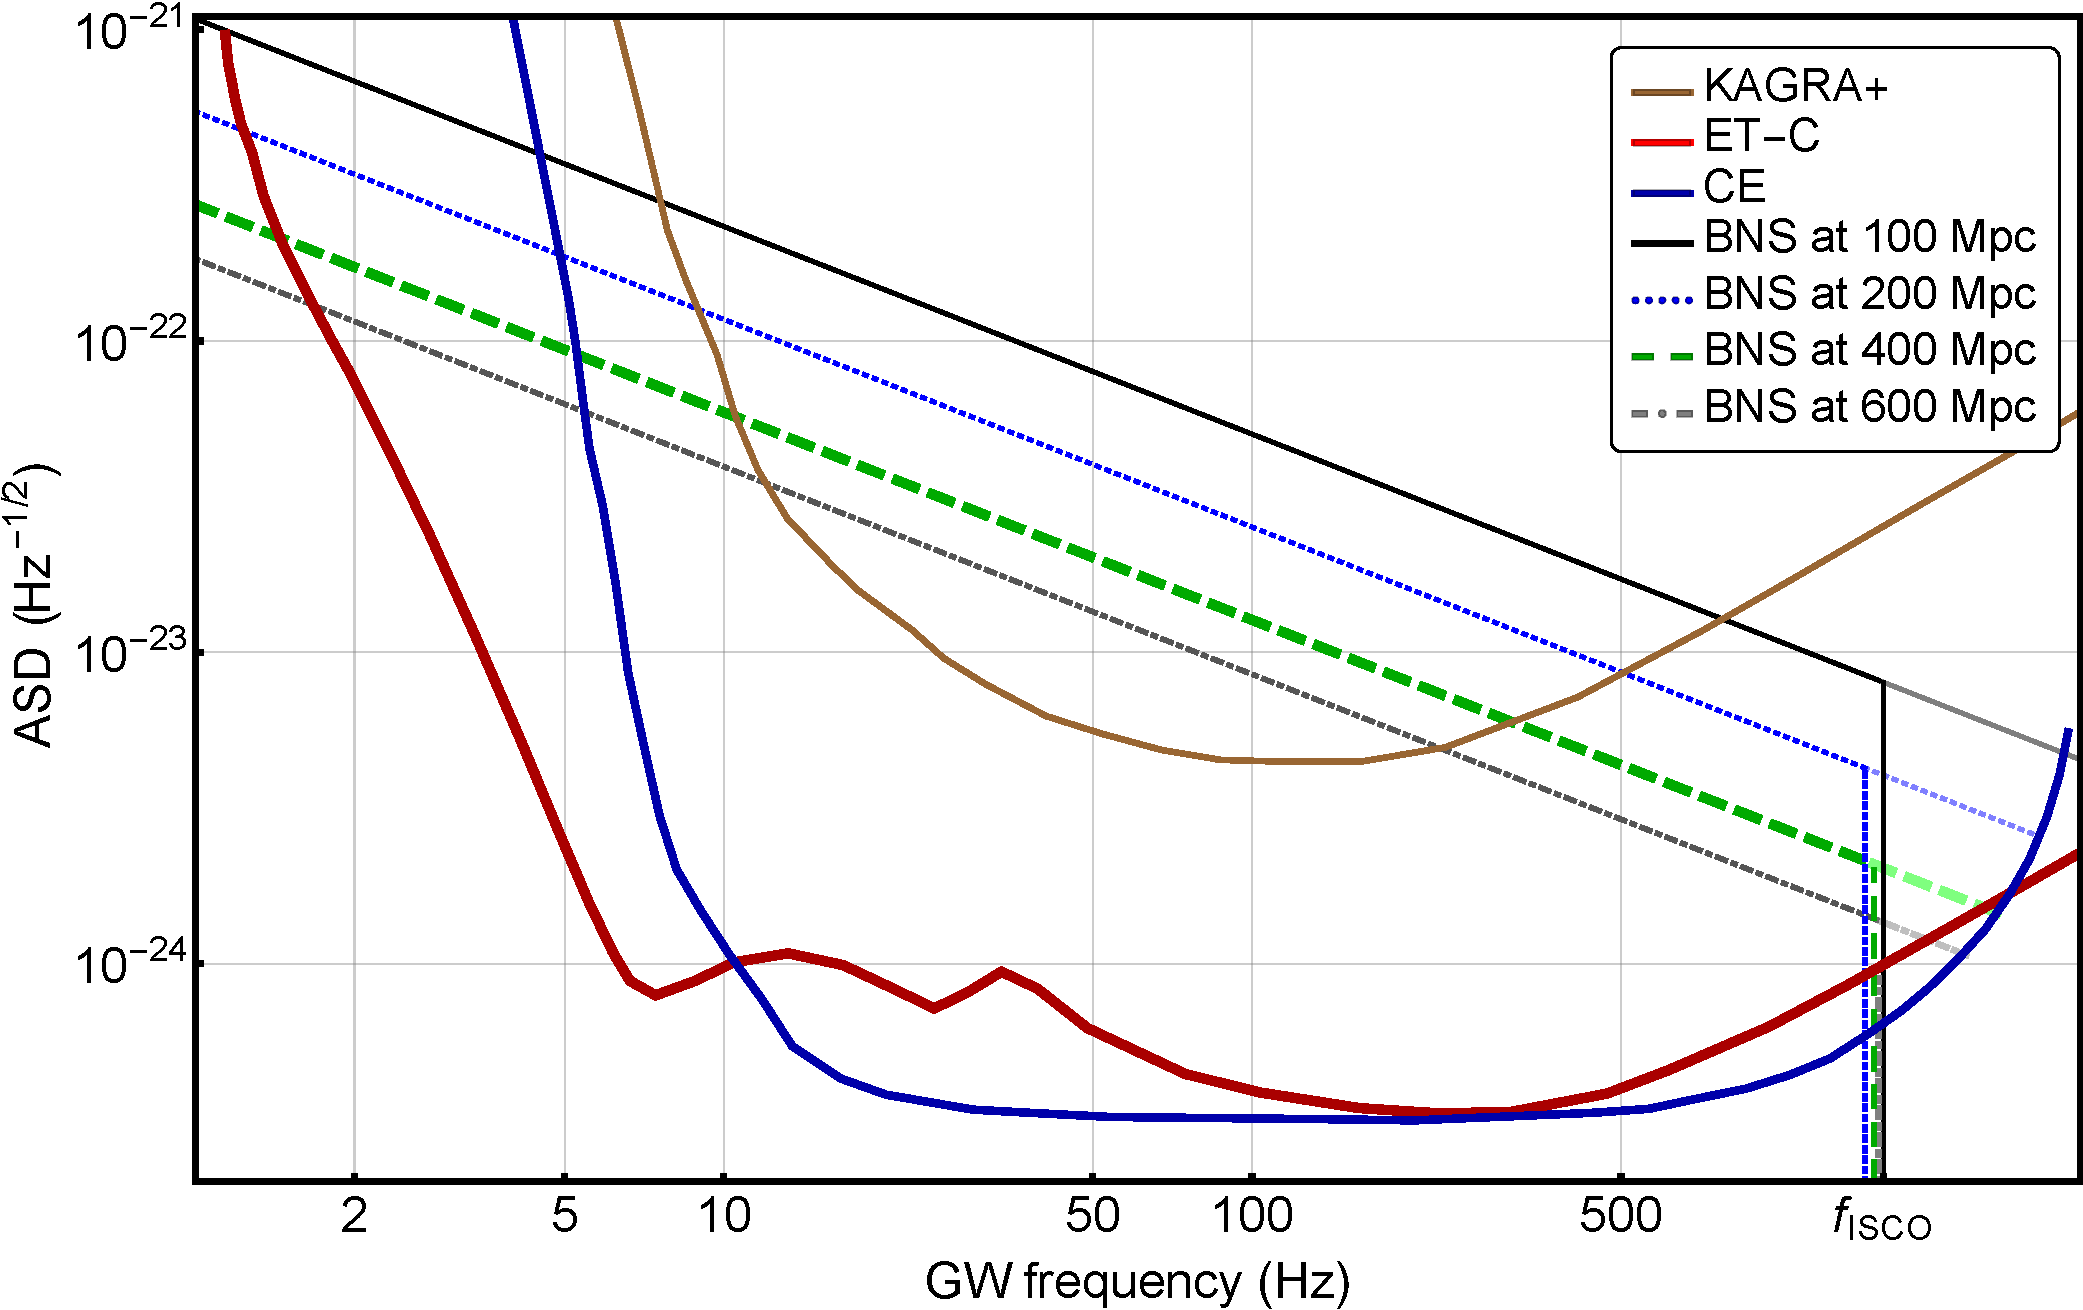
\includegraphics[width=\linewidth]{../Figs/ET_strains_redshifted.pdf}
\caption{Typical GW sources that may be harbingers of GRBs in the 2030s: $1.4 M_\sun-1.4 M_\sun$ inspiralling BNS systems sweeping across 
the Einstein Telescope's sensitivity band for both B and C configurations.
The solid (black), dotted (blue), dashed (green), and dot-dashed lines (gray) lines are the redshift-corrected
RMS-averaged strains, $2\sqrt{f}\tilde{H}_\text{ET}$, at luminosity distances of $D=100, 200, 400, 1000\,$Mpc, respectively. 
The vertical lines with correspondingly identical patterns (colors) mark the redshifted ISCO frequencies $(1+z)^{-1} f_\text{ISCO}$ at which point we terminate each inspiral.
As the true ISCO frequency is likely larger than $f_\text{ISCO}$ cite{Marronetti:2003hx}, the inspirals would continue to nearly 2\,kHz indicated by the 
faded lines in the plot (drawn to 5\,kHz for aesthetic reasons).
%However, numerical simulations indicate that the actual ISCO is smaller than the Schwarzschild value $6GM/c^2$ hence the true ISCO
%frequency is greater than $f_\text{ISCO}$ used here.
%As shown, Einstein Telescope is sensitive enough to accumulate more SNR in this $f>f_\text{ISCO}$ regime.
%Once again, keep in mind that we artificially extended the leading-order $f^{-2/3}$ power law past $f\sim 100\,$Hz at which point tidal effects actually visibly modify this behavior.
}
\label{fig:ETB2030}
\end{figure*}


\section{Implications for optical followup of GW detections} \label{sect:EM}
Identifying an optical or NIR counterpart to a GW is an observational challenge. If a GW is only localised to tens, or even hundreds of square degrees, then we must survey a large area of the sky to find an EM counterpart. While large format CCDs make taking imaging of an area of $\sim$100 sq degrees relatively straightforward, we must identify our EM counterpart of interest among the many unrelated astrophysical transients that we expect by chance within the same area. Thus far, this has relied upon large scale efforts to spectroscopically classify credible candidates that are found within the sky localisation of a GW. As an example, for the BH merger GW151226, \cite{Smar16} found 49 candidate transients within 290 deg$^2$, and obtained spectra for 20 of these. While such a survey strategy is the only feasible approach at present, it is clearly an inefficient use of scarce telescope time.

The early warning obtained for future GW events discussed in Sect. \label{sect:et} offers an alternative approach for finding EM counterparts. In brief, if we can detect a GW with $\sim$1 hr advance warning, and can localise it to $\sim$50 deg$^2$, then we can obtain imaging of this area both immediately prior to, and after, the merger happens. Since the merger will be the only thing that has changed over such a short period of time, identifying an EM counterpart in difference imaging becomes straightforward.

{\bf Morgan:} I would suggest repeating this for $\sim$10 deg$^2$ localisation as well

\subsection{The rates and nature of contaminants}

There are broadly three classes of contaminants that we must consider when searching for EM counterparts to GW; stellar variables and flares such as cataclysmic variables; variability in Active Galactic Nucleii (AGN); and supernovae. The first class of contaminants show a strong dependence on Galactic latitude \citep{Drak14}, and are concentrated in the disk of the Milky Way. In addition, for at least some CV outbursts 

AGN can often be identified through their historical lightcurves, which may show previous variability. Given the relatively straightforward removal of stellar and AGN contaminants, we are left with SNe as the dominant contaminant. Three quarters of SN are SNe Ia in a mag limited survey (cf LOSS). Also, this is borne out by the experience of \cite{Smar16}, where they found...




\begin{figure}[h]
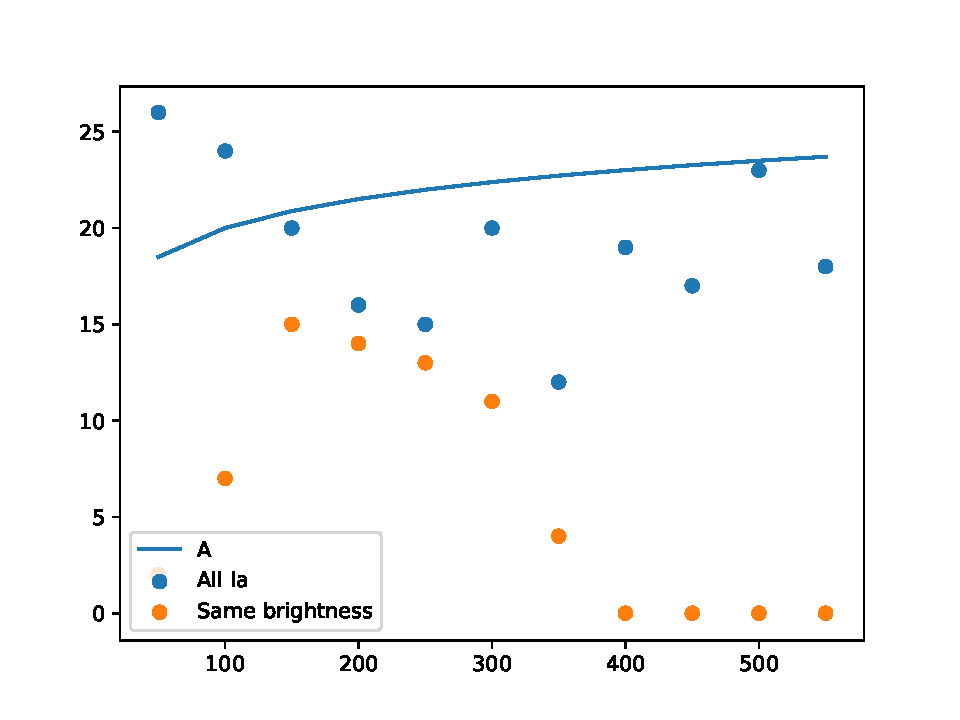
\includegraphics[width=\linewidth]{plot.pdf}
\caption{More or less a placeholder. Number of contaminant SN Ia within our search region as a function of distance...
}
\label{fig:SNIa}
\end{figure}




\begin{acknowledgements}
 SA thanks
\end{acknowledgements}


\bibliographystyle{aa}
\bibliography{GWbib}

\end{document}
